\documentclass[landscape]{article}
\usepackage{geometry} 
\geometry{letterpaper,left=0mm,right=0mm,top=0mm,bottom=0mm,headheight=1mm, footskip=1mm}
\usepackage{fontspec}
\usepackage{tikz}
\setmainfont{Arial}
\usepackage{anyfontsize}
% \usetikzlibrary {shapes.multipart}
% % \setlength\baselineskip{0pt}
% % \setlength\parindent{0pt}
% % \setlength\prevdepth{0pt}
%\newcommand*\mystrut[2]{\vrule height #1 depth #2 width 1pt}


\usetikzlibrary{shapes.geometric}

\tikzset{
  pics/curso/.style args={#1,#2,#3,#4,#5,#6}{
     code={
        \def\ancho{4}
        \def\alto{0.7}
        \draw[fill=#6] (-\ancho/2,\alto) rectangle (\ancho/2,-\alto) node[midway,align=center,text width=4cm]{\fontsize{10pt}{12pt}\selectfont \textbf{#2}};
        \draw[fill=#6] (-\ancho/2,\alto) rectangle (\ancho/2,\alto + \alto) node[midway]{\fontsize{12pt}{14pt}\selectfont #1};
        \draw[fill=#6] (-\ancho/2,-\alto) rectangle (-\ancho/2 + \ancho/3, -\alto - \alto) node[midway]{\fontsize{12pt}{14pt}\selectfont #3};
        \draw[fill=#6] (-\ancho/2 + \ancho/3,-\alto) rectangle (-\ancho/2 + 2*\ancho/3, -\alto - \alto) node[midway]{\fontsize{12pt}{14pt}\selectfont #4};
        \draw[fill=#6] (-\ancho/2 + 2*\ancho/3,-\alto) rectangle (-\ancho/2 + 3*\ancho/3, -\alto - \alto) node[midway]{\fontsize{12pt}{14pt}\selectfont #5};
     }
  }
}

\begin{document}
    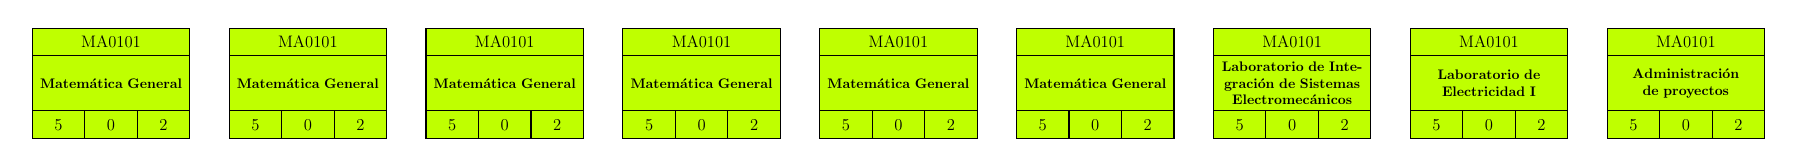
\begin{tikzpicture}[scale=0.5,transform shape]
        \draw (0,0) pic{curso={MA0101,Matemática General,5,0,2,lime}};
        \draw (5,0) pic{curso={MA0101,Matemática General,5,0,2,lime}};
        \draw (10,0) pic{curso={MA0101,Matemática General,5,0,2,lime}};
        \draw (15,0) pic{curso={MA0101,Matemática General,5,0,2,lime}};
        \draw (20,0) pic{curso={MA0101,Matemática General,5,0,2,lime}};
        \draw (25,0) pic{curso={MA0101,Matemática General,5,0,2,lime}};
        \draw (30,0) pic{curso={MA0101,Laboratorio de Integración de Sistemas Electromecánicos,5,0,2,lime}};
        \draw (35,0) pic{curso={MA0101,Laboratorio de Electricidad I,5,0,2,lime}};
        \draw (40,0) pic{curso={MA0101,Administración de proyectos,5,0,2,lime}};
    \end{tikzpicture}
\end{document}

\end{document}